\documentclass[11pt,a4paper]{article}
\usepackage[utf8]{inputenc}
\usepackage[catalan]{babel}
\usepackage{amsmath}
\usepackage{amsfonts}
\usepackage{amssymb}
\usepackage{mathtools}
\usepackage{geometry}
\usepackage{listingsutf8}
\usepackage{listings}
\usepackage{xcolor}
\usepackage{graphicx}
\usepackage{wrapfig}
\usepackage{indentfirst}
\geometry{top=25mm}

\lstset{%language=
                inputencoding=utf8/latin1,
                basicstyle=\ttfamily,
                keywordstyle=\color{blue}\ttfamily,
                stringstyle=\color{red}\ttfamily,
                commentstyle=\color{green}\ttfamily,
                columns=fullflexible,
  frame=single,
  breaklines=true,
  postbreak=\mbox{\textcolor{red}{$\hookrightarrow$}\space},                
                morecomment=[l][\color{magenta}]{\#}
}

\author{Marta Llagostera i Adrià Vilanova\vspace{-2ex} }
\title{Pràctica complementària\vspace{-2ex}}
\date{21 de maig de 2018}
\setlength{\parskip}{1em}
\begin{document}
\maketitle

\section{Problema 1}

\textbf{Objectiu:} Obtenir una estimació de la integral $I = \int_{x_0}^{x_N} f(x) dx$.

Proposem diverses maneres de poder estimar el valor de la integral:

\begin{enumerate}
\item Usant la suma trapeizoïdal
\item Integrant el polinomi de grau $k$ resultat d'aplicar mínims quadrats a la taula de valors
\end{enumerate}

\subsection{Suma trapeizoïdal}

Es tracta de sumar les àrees dels trapecis que tenen una base de longitud $x_i - x_{i-1}$ i dos costats perpendiculars a aquesta base de longitud $f_i$ i $f_{i-1}$, per tot $i \in {1, \ldots, N}$.

\begin{figure}[h]
\centering
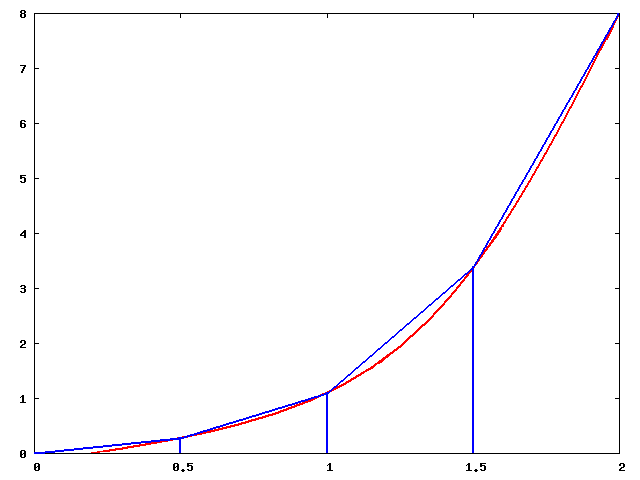
\includegraphics[scale=0.5]{trap}
\caption{Representació visual dels trapecis (creat per Tokigun, domini públic)}
\end{figure}

Així doncs, l'estimació de la integral ens quedaria $I \approx \sum_{i=1}^N (x_i - x_{i-1})\frac{f_i + f_{i-1}}{2} = \frac{1}{2}\sum_{i=1}^N (x_i - x_{i-1})(f_i + f_{i-1})$

\subsection{Mínims quadrats}

Per tal de calcular la integral podem trobar el polinomi que tingui norma mínima (és a dir, el que aproximi millor la funció), i després trobar el valor de la seva integral mitjançant el Teorema Fonamental del Càlcul Integral, ja que és trivial trobar la primitiva d'un polinomi.

Així doncs, si tenim que el polinomi $p(x) = a_0 + a_1 x + a_2 x^2 + \ldots + a_k x^k = \sum_{i=0}^k a_i x^i$ és el polinomi resultat d'aplicar el mètode de mínims quadrats, la seva integral serà $\int_{x_0}^{x_N}p(x)dx = \int_{x_0}^{x_N}\sum_{i=0}^k a_i x^i dx = \left.\sum_{i=0}^k \frac{a_i}{i+1}x^{i+1} \right\rvert_{x_0}^{x_N} = \sum_{i=0}^k \frac{a_i}{i+1}(x_N^{i+1} - x_0^{i+1})$.

\begin{figure}[h]
\centering
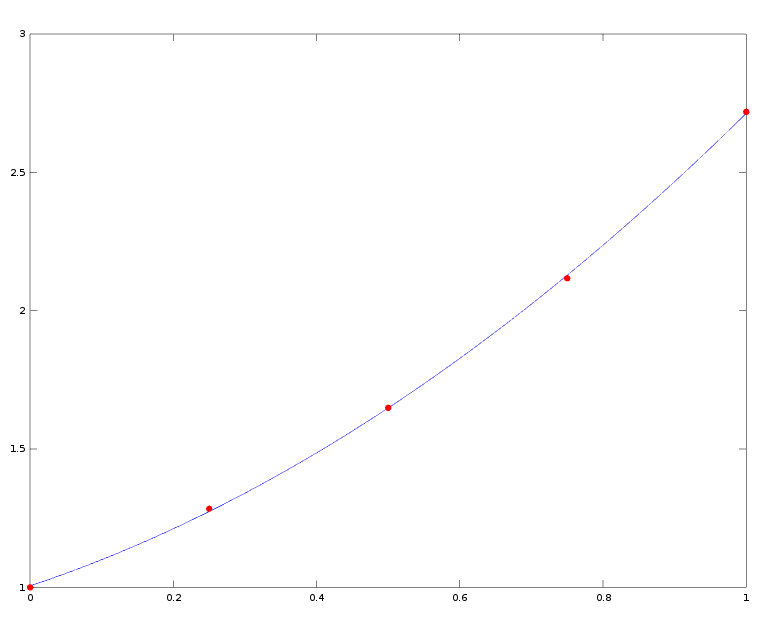
\includegraphics[scale=0.35]{polminquad}
\caption{Un polinomi aproximant una xarxa de punts. En aquest cas, calcularíem la integral definida del polinomi dibuixat en blau.}
\end{figure}

\subsection{Resultats}
Hem fet tres proves: la primera consisteix en estimar $\int_0^1 e^x$ amb una xarxa de 11 punts on $x_i = \frac{i}{10}$. La segona consisteix en estimar la mateixa integral però amb només 5 punts: $x_i = \frac{i}{4}$. La tercera consisteix en estimar $\int_0^1 \sqrt{1-x^2}$ donada una xarxa de 11 punts on $x_i = \frac{i}{10}$.

\subsubsection{Prova 1}

\textbf{Valor de la integral:} $e - 1 \approx 1.71828182845905$

\textbf{Suma trapezoïdal:} 1.71971349138931

\textbf{Mínims quadrats:}

\begin{tabular}{|c|c|}
\hline
\textbf{Grau} & \textbf{Valor estimat} \\
\hline
1 & 1.73238871164751 \\
\hline
2 & 1.71836082773908 \\
\hline
3 & 1.71836082773908 \\
\hline
4 & 1.71828198717880 \\
\hline
5 & 1.71828198717880 \\
\hline
6 & 1.71828182871809 \\
\hline
\end{tabular}

És clar que l'aproximació de la integral feta pel polinomi de grau 2 és millor que la de la suma trapezoïdal.

\subsubsection{Prova 2}

\textbf{Valor de la integral:} $e - 1 \approx 1.71828182845905$

\textbf{Suma trapezoïdal:} 1.72722190455752

\textbf{Mínims quadrats:}

\begin{tabular}{|c|c|}
\hline
\textbf{Grau} & \textbf{Valor estimat} \\
\hline
1 & 1.75360570649192 \\
\hline
2 & 1.71845829305299 \\
\hline
3 & 1.71845829305299 \\
\hline
4 & 1.71828268792475 \\
\hline
5 & 1.25000000000000 \\
\hline
6 & -10127536809625 \\
\hline
\end{tabular}

També està clar que l'aproximació feta pel polinomi de grau 2 és millor que la de la suma trapezoïdal. Observem que el polinomi de grau 6 és una interpolació, i quan la funció que intentem integrar no és polinòmica, això pot resultar en comportaments com aquests, ja que a l'interpolar el polinomi pot prendre valors que no s'aproximen res a la nostra funció no polinòmica.

\subsubsection{Prova 3}

\textbf{Valor de la integral:} $\int_0^1 \sqrt{1-x^2} = \pi / 4 \approx 0.785398163397448$

\textbf{Suma trapezoïdal:} 1.71971349138931

\textbf{Mínims quadrats:}

\begin{tabular}{|c|c|}
\hline
\textbf{Grau} & \textbf{Valor estimat} \\
\hline
1 & 0.751026892329163 \\
\hline
2 & 0.774554309700456 \\
\hline
3 & 0.774554309700456 \\
\hline
4 & 0.780068770351144 \\
\hline
5 & 0.780068770351143 \\
\hline
6 & 0.781782050231272 \\
\hline
\end{tabular}

De nou l'aproximació que fem amb el polinomi de mínims quadrats és millor que la suma trapezoïdal inclús quan aproximem la funció per una recta.

En conclusió, podríem dir que el mètode de mínims quadrats és millor que el de la suma trapezoïdal.

\section{Problema 2}

Quan tenim petits errors a les dades d'entrada per resoldre un sistema d'equacions $Ax = b$, a vegades els resultats poden arribar a ser molt imprecisos. Per tal d'evitar això, podem observar un nombre especial anomenat el nombre de condició ($\mu(A) = ||A^{-1}||\cdot||A||$). Aquest nombre representa el factor màxim d'amplificació dels errors relatius de les dades d'entrada: la matriu $A$ i el vector $b$. Aquest nombre ens dóna una fita de l'error relatiu (si suposem $|| x + \delta x || \approx ||x||$):

$\frac{||\delta x||}{||x||} \leq \mu(A) [\frac{||\delta b||}{||b||} + \frac{||\delta A||}{||A||}]$

Així doncs, sempre ens interessa que aquest nombre sigui proper a 1, ja que això ens garanteix que els errors a les dades no es percebran a la sortida.

Malhauradament, les matrius de Hilbert són matrius simètriques definides positives que, en general (exceptuant $n$s petites), tenen nombres de condició molt grans.

El fet que al tractar de resoldre el sistema numèricament hi ha errors d'arrodoniment a l'entrada i mentre es fan els càlculs juntament amb el fet que els errors es poden propagar molt ràpidament, fa que l'error que hi ha a la sortida sigui molt gran. De fet, això empitjora quan $n$ és més gran.

A la següent gràfica es pot observar que el nombre de condició ($A_n$) està directament relacionat amb l'error relatiu de la solució del sistema ($E_n$). També està representat l'error al calcular la descomposició LU ($R_n = ||PA - LU||_{\infty}$).

\begin{center}
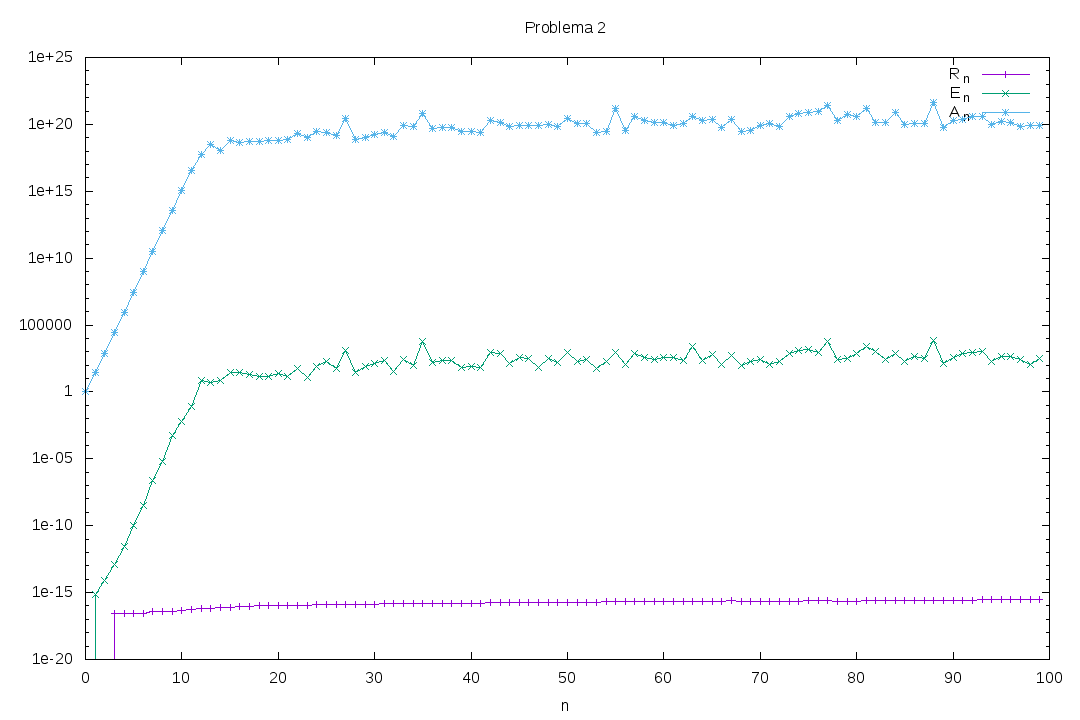
\includegraphics[scale=0.4]{grafica}
\end{center}

Així doncs, també podem veure a la gràfica que tot i que la descomposició LU està feta quasi perfectament, ja que el residu $R_n$ és d'un ordre molt petit, la solució no és la esperada per $n$s molt grans.

\end{document}